\documentclass{my_class}
% ==============================================================================
% Academic Document LaTeX Template
% Author: Marco Tijbout
% License: Creative Commons Attribution-NonCommercial-ShareAlike 4.0 International (CC BY-NC-SA 4.0)
% ------------------------------------------------------------------------------
% You are free to share, adapt, and modify this template for personal and 
% academic purposes, provided that:
%   1. Attribution is given ("Based on the template by Marco Tijbout").
%   2. It is not used for commercial purposes or resold.
%   3. Any derivative versions are distributed under the same license (CC BY-NC-SA 4.0).
% 
% For full license details, visit: https://creativecommons.org/licenses/by-nc-sa/4.0/
% ==============================================================================

\addbibresource{references.bib}

\title{This is the title of the report}
\author{Author Name}
\date{July 2026}

\institution{University of ABCD Online}
\affiliation{at  EFGH College Z\"urich}
\reporttype{This describes the report type --- Part N}
\coursename{This is the name of the course}
\gnumber{G12345678}
\supervisor{Name Professor }
\degreetitle{Master of Science in Artificial Intelligence}

\newacronym{ml}{ML}{Machine Learning}
\newacronym{ai}{AI}{Artificial Intelligence}
\newacronym{api}{API}{Application Programming Interface}

\begin{document}
	
% --- Begin of the document section ---	
	% !TEX root = ../main.tex
% Custom title page, replacing the default \maketitle output.
% Fields (\title, \author, \date, \institution, etc.) are set in
% main.tex before this file is \input.

\makeatletter
\begin{titlepage}
    \centering

    {\Large \@institution \par}
    \vspace{0.2cm}
    {\large \@affiliation \par}

    \vspace{1cm}
    \rule{\linewidth}{0.6pt}
    \vspace{0.8cm}

    {\huge\bfseries \@title \par}

    \vspace{0.8cm}
    \rule{\linewidth}{0.6pt}
    \vspace{0.5cm}

    {\Large \@reporttype \par}
    \vspace{0.3cm}
    {\large \@coursename \par}

    \vspace{2.5cm}

    {\Large \MakeUppercase{\@author} \par}
    \vspace{0.3cm}
    {\normalsize G Number: \@gnumber \par}
    \vspace{0.2cm}
    {\normalsize Supervisor: \MakeUppercase {\@supervisor} \par}

    \vfill

    {\normalsize Submitted in partial satisfaction of the requirements for the degree of \par}
    \vspace{0.2cm}
    {\normalsize \@degreetitle \par}

    \vspace{1cm}
    {\normalsize \@date \par}

\end{titlepage}
\makeatother

	% !TEX root = ../main.tex

\chapter*{Declaration}
\addcontentsline{toc}{chapter}{Declaration}

I declare that all material contained in this report, including ideas described in the
text, computer programs and drawings, is my own work except where explicitly and
individually acknowledged.

\vspace{2cm}

\noindent Signed \dotfill

\vspace{1cm}

\noindent Date \dotfill

	% !TEX root = ../main.tex

\chapter*{Abstract}
\addcontentsline{toc}{chapter}{Abstract}

Lorem ipsum dolor sit amet, consetetur sadipscing elitr, sed diam nonumy eirmod tempor invidunt ut labore et dolore magna aliquyam erat, sed diam voluptua. At vero eos et accusam et justo duo dolores et ea rebum. Stet clita kasd gubergren, no sea takimata sanctus est Lorem ipsum dolor sit amet. Lorem ipsum dolor sit amet, consetetur sadipscing elitr, sed diam nonumy eirmod tempor invidunt ut labore et dolore magna aliquyam erat, sed diam voluptua. At vero eos et accusam et justo duo dolores et ea rebum. Stet clita kasd gubergren, no sea takimata sanctus est Lorem ipsum dolor sit amet. Lorem ipsum dolor sit amet, consetetur sadipscing elitr, sed diam nonumy eirmod tempor invidunt ut labore et dolore magna aliquyam erat, sed diam voluptua. At vero eos et accusam et justo duo dolores et ea rebum. Stet clita kasd gubergren, no sea takimata sanctus est Lorem ipsum dolor sit amet.

Duis autem vel eum iriure dolor in hendrerit in vulputate velit esse molestie consequat, vel illum dolore eu feugiat nulla facilisis at vero eros et accumsan et iusto odio dignissim qui blandit praesent luptatum zzril delenit augue duis dolore te feugait nulla facilisi. Lorem ipsum dolor sit amet, consectetuer adipiscing elit, sed diam nonummy nibh euismod tincidunt ut laoreet dolore magna aliquam erat volutpat.

Ut wisi enim ad minim veniam, quis nostrud exerci tation ullamcorper suscipit lobortis nisl ut aliquip ex ea commodo consequat. Duis autem vel eum iriure dolor in hendrerit in vulputate velit esse molestie consequat, vel illum dolore eu feugiat nulla facilisis at vero eros et accumsan et iusto odio dignissim qui blandit praesent luptatum zzril delenit augue duis dolore te feugait nulla facilisi.

Nam liber tempor cum soluta nobis eleifend option congue nihil imperdiet doming id quod mazim placerat facer possim assum. Lorem ipsum dolor sit amet, consectetuer adipiscing elit, sed diam nonummy nibh euismod tincidunt ut laoreet dolore magna aliquam erat volutpat. Ut wisi enim ad minim veniam, quis nostrud exerci tation ullamcorper suscipit lobortis nisl ut aliquip ex ea commodo consequat.

Duis autem vel eum iriure dolor in hendrerit in vulputate velit esse molestie consequat, vel illum dolore eu feugiat nulla facilisis. 


	\tableofcontents
	\listoffigures
	\listoftables
	
	% !TEX root = ../main.tex

\chapter{Introduction}

Lorem ipsum dolor sit amet, consetetur sadipscing elitr, sed diam nonumy eirmod tempor invidunt ut labore et dolore magna aliquyam erat, sed diam voluptua. At vero eos et accusam et justo duo dolores et ea rebum. Stet clita kasd gubergren, no sea takimata sanctus est Lorem ipsum dolor sit amet. Lorem ipsum dolor sit amet, consetetur sadipscing elitr, sed diam nonumy eirmod tempor invidunt ut labore et dolore magna aliquyam erat, sed diam voluptua. At vero eos et accusam et justo duo dolores et ea rebum. Stet clita kasd gubergren, no sea takimata sanctus est Lorem ipsum dolor sit amet. Lorem ipsum dolor sit amet, consetetur sadipscing elitr, sed diam nonumy eirmod tempor invidunt ut labore et dolore magna aliquyam erat, sed diam voluptua. At vero eos et accusam et justo duo dolores et ea rebum. Stet clita kasd gubergren, no sea takimata sanctus est Lorem ipsum dolor sit amet.

Duis autem vel eum iriure dolor in hendrerit in vulputate velit esse molestie consequat, vel illum dolore eu feugiat nulla facilisis at vero eros et accumsan et iusto odio dignissim qui blandit praesent luptatum zzril delenit augue duis dolore te feugait nulla facilisi. Lorem ipsum dolor sit amet, consectetuer adipiscing elit, sed diam nonummy nibh euismod tincidunt ut laoreet dolore magna aliquam erat volutpat.

Ut wisi enim ad minim veniam, quis nostrud exerci tation ullamcorper suscipit lobortis nisl ut aliquip ex ea commodo consequat. Duis autem vel eum iriure dolor in hendrerit in vulputate velit esse molestie consequat, vel illum dolore eu feugiat nulla facilisis at vero eros et accumsan et iusto odio dignissim qui blandit praesent luptatum zzril delenit augue duis dolore te feugait nulla facilisi.
	% !TEX root = ../main.tex

\chapter{Methodology}

Duis autem vel eum iriure dolor in hendrerit in vulputate velit esse molestie consequat, vel illum dolore eu feugiat nulla facilisis at vero eros et accumsan et iusto odio dignissim qui blandit praesent luptatum zzril delenit augue duis dolore te feugait nulla facilisi. Lorem ipsum dolor sit amet, consectetuer adipiscing elit, sed diam nonummy nibh euismod tincidunt ut laoreet dolore magna aliquam erat volutpat.

\section{Lorem ipsum dolor}
Lorem ipsum dolor sit amet, consetetur sadipscing elitr, sed diam nonumy eirmod tempor invidunt ut labore et dolore magna aliquyam erat, sed diam voluptua. At vero eos et accusam et justo duo dolores et ea rebum. Stet clita kasd gubergren, no sea takimata sanctus est Lorem ipsum dolor sit amet. Lorem ipsum dolor sit amet, consetetur sadipscing elitr, sed diam nonumy eirmod tempor invidunt ut labore et dolore magna aliquyam erat, sed diam voluptua. At vero eos et accusam et justo duo dolores et ea rebum. Stet clita kasd gubergren, no sea takimata sanctus est Lorem ipsum dolor sit amet. Lorem ipsum dolor sit amet, consetetur sadipscing elitr, sed diam nonumy eirmod tempor invidunt ut labore et dolore magna aliquyam erat, sed diam voluptua. At vero eos et accusam et justo duo dolores et ea rebum. Stet clita kasd gubergren, no sea takimata sanctus est Lorem ipsum dolor sit amet.

\section{Ut wisi enim}
Ut wisi enim ad minim veniam, quis nostrud exerci tation ullamcorper suscipit lobortis nisl ut aliquip ex ea commodo consequat. Duis autem vel eum iriure dolor in hendrerit in vulputate velit esse molestie consequat, vel illum dolore eu feugiat nulla facilisis at vero eros et accumsan et iusto odio dignissim qui blandit praesent luptatum zzril delenit augue duis dolore te feugait nulla facilisi.

\section{Duis autem vel}
Nam liber tempor cum soluta nobis eleifend option congue nihil imperdiet doming id quod mazim placerat facer possim assum. Lorem ipsum dolor sit amet, consectetuer adipiscing elit, sed diam nonummy nibh euismod tincidunt ut laoreet dolore magna aliquam erat volutpat. Ut wisi enim ad minim veniam, quis nostrud exerci tation ullamcorper suscipit lobortis nisl ut aliquip ex ea commodo consequat.
	% !TEX root = ../main.tex

\chapter{Results}

Write your results here.

Lorem ipsum dolor sit amet, consetetur sadipscing elitr, sed diam nonumy eirmod tempor invidunt ut labore et dolore magna aliquyam erat, sed diam voluptua. At vero eos et accusam et justo duo dolores et ea rebum. Stet clita kasd gubergren, no sea takimata sanctus est Lorem ipsum dolor sit amet. Lorem ipsum dolor sit amet, consetetur sadipscing elitr, sed diam nonumy eirmod tempor invidunt ut labore et dolore magna aliquyam erat, sed diam voluptua. At vero eos et accusam et justo duo dolores et ea rebum. Stet clita kasd gubergren, no sea takimata sanctus est Lorem ipsum dolor sit amet. Lorem ipsum dolor sit amet, consetetur sadipscing elitr, sed diam nonumy eirmod tempor invidunt ut labore et dolore magna aliquyam erat, sed diam voluptua. At vero eos et accusam et justo duo dolores et ea rebum. Stet clita kasd gubergren, no sea takimata sanctus est Lorem ipsum dolor sit amet.

Duis autem vel eum iriure dolor in hendrerit in vulputate velit esse molestie consequat, vel illum dolore eu feugiat nulla facilisis at vero eros et accumsan et iusto odio dignissim qui blandit praesent luptatum zzril delenit augue duis dolore te feugait nulla facilisi. Lorem ipsum dolor sit amet, consectetuer adipiscing elit, sed diam nonummy nibh euismod tincidunt ut laoreet dolore magna aliquam erat volutpat.
	% !TEX root = ../main.tex

\chapter{Conclusion}

Write your conclusion here.

Lorem ipsum dolor sit amet, consetetur sadipscing elitr, sed diam nonumy eirmod tempor invidunt ut labore et dolore magna aliquyam erat, sed diam voluptua. At vero eos et accusam et justo duo dolores et ea rebum. Stet clita kasd gubergren, no sea takimata sanctus est Lorem ipsum dolor sit amet. Lorem ipsum dolor sit amet, consetetur sadipscing elitr, sed diam nonumy eirmod tempor invidunt ut labore et dolore magna aliquyam erat, sed diam voluptua. At vero eos et accusam et justo duo dolores et ea rebum. Stet clita kasd gubergren, no sea takimata sanctus est Lorem ipsum dolor sit amet. Lorem ipsum dolor sit amet, consetetur sadipscing elitr, sed diam nonumy eirmod tempor invidunt ut labore et dolore magna aliquyam erat, sed diam voluptua. At vero eos et accusam et justo duo dolores et ea rebum. Stet clita kasd gubergren, no sea takimata sanctus est Lorem ipsum dolor sit amet.

Duis autem vel eum iriure dolor in hendrerit in vulputate velit esse molestie consequat, vel illum dolore eu feugiat nulla facilisis at vero eros et accumsan et iusto odio dignissim qui blandit praesent luptatum zzril delenit augue duis dolore te feugait nulla facilisi. Lorem ipsum dolor sit amet, consectetuer adipiscing elit, sed diam nonummy nibh euismod tincidunt ut laoreet dolore magna aliquam erat volutpat.

Ut wisi enim ad minim veniam, quis nostrud exerci tation ullamcorper suscipit lobortis nisl ut aliquip ex ea commodo consequat. Duis autem vel eum iriure dolor in hendrerit in vulputate velit esse molestie consequat, vel illum dolore eu feugiat nulla facilisis at vero eros et accumsan et iusto odio dignissim qui blandit praesent luptatum zzril delenit augue duis dolore te feugait nulla facilisi.

Nam liber tempor cum soluta nobis eleifend option congue nihil imperdiet doming id quod mazim placerat facer possim assum. Lorem ipsum dolor sit amet, consectetuer adipiscing elit, sed diam nonummy nibh euismod tincidunt ut laoreet dolore magna aliquam erat volutpat. Ut wisi enim ad minim veniam, quis nostrud exerci tation ullamcorper suscipit lobortis nisl ut aliquip ex ea commodo consequat.

Duis autem vel eum iriure dolor in hendrerit in vulputate velit esse molestie consequat, vel illum dolore eu feugiat nulla facilisis. 

At vero eos et accusam et justo duo dolores et ea rebum. Stet clita kasd gubergren, no sea takimata sanctus est Lorem ipsum dolor sit amet. Lorem ipsum dolor sit amet, consetetur sadipscing elitr, sed diam nonumy eirmod tempor invidunt ut labore et dolore magna aliquyam erat, sed diam voluptua. At vero eos et accusam et justo duo dolores et ea rebum. Stet clita kasd gubergren, no sea takimata sanctus est Lorem ipsum dolor sit amet. Lorem ipsum dolor sit amet, consetetur sadipscing elitr, At accusam aliquyam diam diam dolore dolores duo eirmod eos erat, et nonumy sed tempor et et invidunt justo labore Stet clita ea et gubergren, kasd magna no rebum. sanctus sea sed takimata ut vero voluptua. est Lorem ipsum dolor sit amet. Lorem ipsum dolor sit amet, consetetur sadipscing elitr, sed diam nonumy eirmod tempor invidunt ut labore et dolore magna aliquyam erat.
	% !TEX root = ../main.tex

\chapter{Template}

Write your template examples here.

\begin{figure}[htbp]
	\centering
	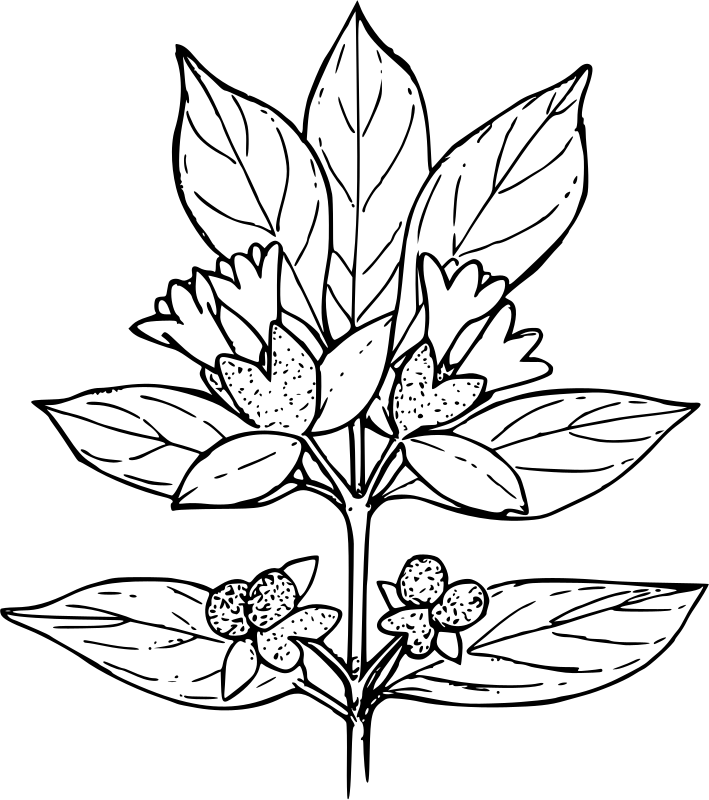
\includegraphics[width=0.8\textwidth]{figures/flower.png}
	\caption{Description of the flower.}
	\label{fig:flower}
\end{figure}



We have some text before the inserted PDF ...

% --- Importing PDF files
% Imported a specific page of a pdf file
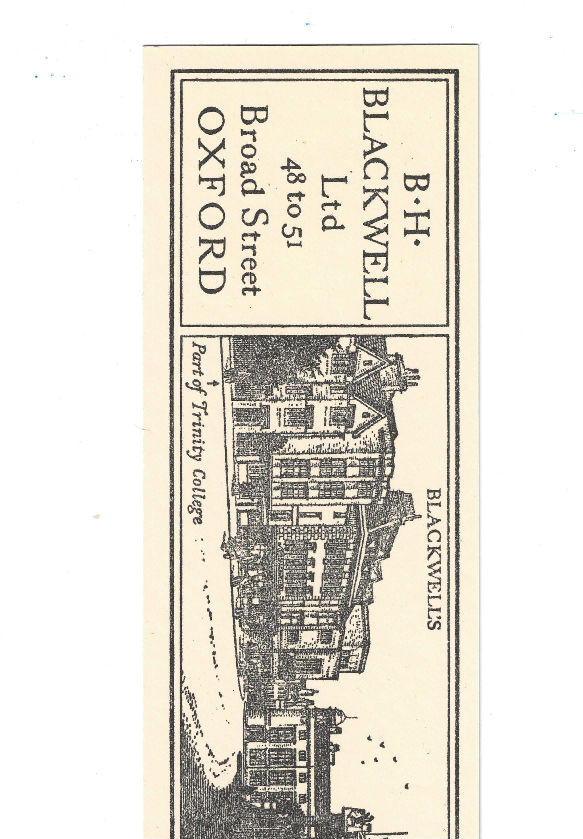
\includepdf[pages=1]{figures/example1v.pdf}

% --- All pages:
% \includepdf[pages=-]{figures/report_appendix.pdf}

% --- Specific pages with a fitting mode:
% \includepdf[pages={2,4-6}, fitpaper=true]{figures/document.pdf}

We have some text after the inserted PDF ...

\section{Example Table}

Table~\ref{tab:example} shows a simple comparison.

\begin{table}[htbp]
	\centering
	\caption{Comparison of example values.}
	\label{tab:example}
	\begin{tabular}{lcc}
		\toprule
		\textbf{Category} & \textbf{Value A} & \textbf{Value B} \\
		\midrule
		Alpha  & 12.4 & 8.1  \\
		Beta   & 9.7  & 14.3 \\
		Gamma  & 15.2 & 11.6 \\
		\bottomrule
	\end{tabular}
\end{table}

\section{Example Citation}

Bias in machine learning models often originates from unbalanced training data
rather than flawed algorithms \citep{smith2021}. As Smith and Jones (2021)
demonstrate \citep{smith2021}, this distinction has significant implications
for how practitioners approach model auditing.

\Gls{ai} is one of the most disruptive technologies.


\section{Example Lists}

\subsection{Bulleted List}

An unordered list is useful when items have no inherent sequence:

\begin{itemize}
	\item First point of consideration.
	\item Second point, independent of the first.
	\item Third point, with a nested sub-list:
	\begin{itemize}
		\item Sub-point A.
		\item Sub-point B.
	\end{itemize}
\end{itemize}

\subsection{Numbered List}

An ordered list is useful when sequence or ranking matters:

\begin{enumerate}
	\item Initial step of the process.
	\item Subsequent step, dependent on the first.
	\item Final step, concluding the sequence.
\end{enumerate}

\subsection{Description List}

A description list pairs a term with its explanation — useful for glossaries or defining terms:

\begin{description}
	\item[Bias] Systematic error introduced into a model due to unrepresentative training data.
	\item[Variance] Sensitivity of a model to small fluctuations in the training set.
	\item[Overfitting] A model that captures noise rather than underlying patterns.
\end{description}

% Referencing to online content on a website:
Recent evidence suggests pandemic-related isolation significantly increased
reported anxiety and depressive symptoms globally \citep{who2023}.

Model training in this project made use of the scikit-learn library
\citep{pedregosa2011}.

The Transformer architecture dispensed with recurrence entirely, relying
solely on attention mechanisms \citep{vaswani2017}. \\

\Gls{ml} models require large datasets.
% First occurrence renders as: "Machine Learning (ML) models require large datasets."
% Any subsequent \gls{ml} renders as just: "ML models require large datasets."

\Gls{api} adds the capability for subcomponents of an application to communicate with each other.

\Gls{ai} is one of the most disruptive technologies.

% -----------------------------------------------------------------
% LONG TABLES (crossing multiple pages)
% -----------------------------------------------------------------
% The standard `tabular` environment (used in the table examples
% above) does NOT break across pages — if content overflows, it
% either gets cut off or throws an overfull box warning.
%
% For tables that may span multiple pages (e.g. long datasets,
% detailed appendix listings), use `longtable` instead.
%
% REQUIRES: \RequirePackage{longtable} in mycls.cls (not yet added
% — add it if you use this).
%
% KEY DIFFERENCES FROM `tabular`:
%   - No \begin{table}...\end{table} wrapper — longtable is a
%     floating-like environment on its own; wrapping it in `table`
%     will break page-splitting.
%   - Caption and label go INSIDE the longtable environment, not
%     around it.
%   - \endhead marks header rows that repeat on every page.
%   - \endfoot / \endlastfoot let you define a footer that differs
%     on the final page (e.g. "continued on next page" vs a closing
%     \bottomrule).
%
% EXAMPLE:
%
% \begin{longtable}{ll}
	%     \caption{Overview of submitted files.} \label{tab:submitted-files} \\
	%     \toprule
	%     \textbf{File} & \textbf{Description} \\
	%     \midrule
	%     \endfirsthead
	%
	%     % Header repeated on subsequent pages:
	%     \multicolumn{2}{l}{\small\itshape (continued from previous page)} \\
	%     \toprule
	%     \textbf{File} & \textbf{Description} \\
	%     \midrule
	%     \endhead
	%
	%     % Footer on all pages except the last:
	%     \midrule
	%     \multicolumn{2}{r}{\small\itshape continued on next page} \\
	%     \endfoot
	%
	%     % Footer on the final page only:
	%     \bottomrule
	%     \endlastfoot
	%
	%     \texttt{main.pdf}       & Compiled report (this document). \\
	%     \texttt{main.tex}       & Main LaTeX source file.          \\
	%     % ... more rows ...
	%
	% \end{longtable}
%
% NOTE: longtable disables centering by default — wrap in
% \begin{center}...\end{center} if needed, or use the `ltcaption`
% package's alignment options.
% -----------------------------------------------------------------

\section{Example Long Table}

Table~\ref{tab:long-example} demonstrates a table spanning multiple pages,
with the header row repeating automatically on each page.

\begin{longtable}{ll}
	\longtablecaption{Example long table spanning multiple pages.}{tab:long-example}
	\toprule
	\textbf{Item} & \textbf{Value} \\
	\midrule
	\endfirsthead
	
	\multicolumn{2}{l}{\small\itshape (continued from previous page)} \\
	\toprule
	\textbf{Item} & \textbf{Value} \\
	\midrule
	\endhead
	
	\midrule
	\multicolumn{2}{r}{\small\itshape continued on next page} \\
	\endfoot
	
	\bottomrule
	\endlastfoot
	
	Entry 01 & 12.4 \\
	Entry 02 & 8.1  \\
	Entry 03 & 15.2 \\
	Entry 04 & 9.7  \\
	Entry 05 & 14.3 \\
	Entry 06 & 11.6 \\
	Entry 07 & 13.8 \\
	Entry 08 & 10.5 \\
	Entry 09 & 16.1 \\
	Entry 10 & 7.9  \\
	Entry 11 & 12.0 \\
	Entry 12 & 14.7 \\
	Entry 13 & 9.3  \\
	Entry 14 & 15.9 \\
	Entry 15 & 11.2 \\
	Entry 16 & 13.4 \\
	Entry 17 & 8.6  \\
	Entry 18 & 16.8 \\
	Entry 19 & 10.1 \\
	Entry 20 & 12.9 \\
	Entry 21 & 14.2 \\
	Entry 22 & 9.8  \\
	Entry 23 & 15.5 \\
	Entry 24 & 11.7 \\
	Entry 25 & 13.1 \\
	Entry 26 & 8.4  \\
	Entry 27 & 16.3 \\
	Entry 28 & 10.9 \\
	Entry 29 & 12.6 \\
	Entry 30 & 14.9 \\
Entry 01 & 12.4 \\
Entry 02 & 8.1  \\
Entry 03 & 15.2 \\
Entry 04 & 9.7  \\
Entry 05 & 14.3 \\
Entry 06 & 11.6 \\
Entry 07 & 13.8 \\
Entry 08 & 10.5 \\
Entry 09 & 16.1 \\
Entry 10 & 7.9  \\
Entry 11 & 12.0 \\
Entry 12 & 14.7 \\
Entry 13 & 9.3  \\
Entry 14 & 15.9 \\
Entry 15 & 11.2 \\
Entry 16 & 13.4 \\
Entry 17 & 8.6  \\
Entry 18 & 16.8 \\
Entry 19 & 10.1 \\
Entry 20 & 12.9 \\
Entry 21 & 14.2 \\
Entry 22 & 9.8  \\
Entry 23 & 15.5 \\
Entry 24 & 11.7 \\
Entry 25 & 13.1 \\
Entry 26 & 8.4  \\
Entry 27 & 16.3 \\
Entry 28 & 10.9 \\
Entry 29 & 12.6 \\
Entry 30 & 14.9 \\
\end{longtable}




% --- End of the document section ---

% --- Begin of any appendices at the end of the document.
	
	\appendix
	\printbibliography[title={References}, heading=bibintoc]  % Making sure it is listed in the TOC
	\printglossary[type=\acronymtype, title={List of Abbreviations}]		
	% !TEX root = ../main.tex

\chapter{Submitted Files}

Table~\ref{tab:submitted-files} lists the files submitted alongside this report.

\begin{table}[htbp]
	\centering
	\caption{Overview of submitted files.}
	\label{tab:submitted-files}
	\begin{tabular}{ll}
		\toprule
		\textbf{File} & \textbf{Description} \\
		\midrule
		\texttt{main.pdf}            & Compiled report (this document).        \\
		\texttt{main.tex}            & Main LaTeX source file.                 \\
		\texttt{references.bib}      & Bibliography source file.               \\
		\texttt{mycls.cls}           & Custom document class.                  \\
		\texttt{chapters/}           & Folder containing chapter source files. \\
		\texttt{figures/}            & Folder containing images and PDFs used. \\
		\bottomrule
	\end{tabular}
\end{table}



% --- End of any appendices 	
\end{document}